\documentclass{report}
\usepackage{titlesec}
\usepackage[T1]{fontenc}
\usepackage[utf8]{inputenc}
\usepackage[backend=biber, style=ieee]{biblatex}
\usepackage{csquotes}
\usepackage[portuguese]{babel}
\usepackage{blindtext}
\usepackage[printonlyused]{acronym}
\usepackage{hyperref}
\usepackage{graphicx}
\usepackage{indentfirst}
\usepackage{tabularx}
\usepackage{float}
\usepackage{subcaption}

\setlength{\parskip}{0.39em}
\titleformat{\section}{\normalfont\huge}{\thechapter.}{20pt}{\huge\bf}
\newcommand{\centered}[1]{\begin{tabular}{l} #1 \end{tabular}}

\begin{document}
%%% DEFINIÇÕES GLOBAIS %%%
\def\titulo{Filtro de Média Móvel}
\def\data{Aveiro, junho 2022}
\def\autores{Luíz Fernando, Miguel Vila}
\def\autorescontactos{(107535) \href{mailto:luiz.ferreira@ua.pt}{luiz.ferreira@ua.pt}, (107276) \href{mailto:miguelovila@ua.pt}{miguelovila@ua.pt}}
\def\disciplina{Laboratório de Sistemas Digitais}
\def\instituicao{UNIVERSIDADE DE AVEIRO}

%%%  PÁGINA DE TÍTULO %%%
\title{%
{\Huge\textbf{\titulo}}\\
{\Large \disciplina\\}
}
\author{
    \autores \\
    \autorescontactos \\\\
    \instituicao
}
\date{\data}
\maketitle
\pagenumbering{roman}

%%% INTRODUÇÃO %%%%
\section*{Introdução}
\label{chap.introducao}

Para este trabalho foi proposto o desenvolvimento de um filtro de média móvel, um componente frequente em sistemas de processamento de sinal e ou imagem, responsável pela suavização de um sinal de entrada na FPGA Terasic DE2-115.

Este filtro, de largura 4, irá suavizar um sinal de entrada disponível numa ROM de 256x8 bits. Já o sinal de saída deverá ser guardado numa RAM com as mesmas dimensões.

\section*{Manual de Utilização}
\label{chap.manualdeutilizacao}

\begin{figure}[H]
    \centering
    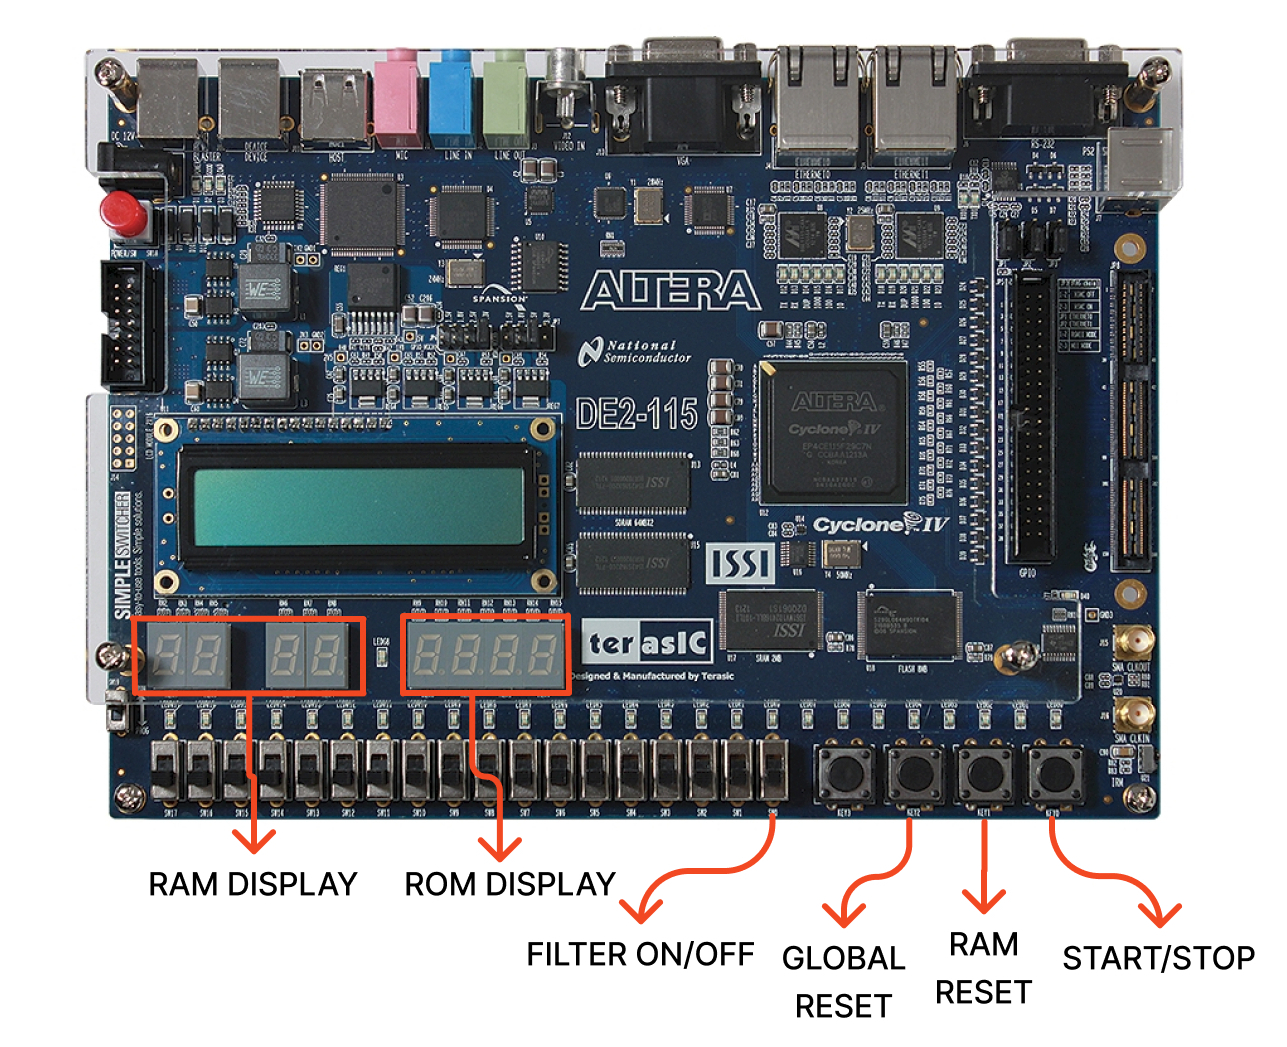
\includegraphics[width=\textwidth]{fpga.jpg}
    \caption{Funções e visualização de dados na Terasic DE2-115}
\end{figure}

O filtro possui as seguintes funcionalidades:
\begin{itemize}
    \item RAM Display: é onde pode ser feita a visualização dos valores guardados na memória RAM no endereço atual.
    \item ROM Display: é onde pode ser feita a visualização do valor presente na memória ROM no endereço atual.
    \item Filter ON/OFF: caso esteja ligado, o valor armazenado na memória RAM resulta de uma média entre os dois valores anteriores, o valor atual e o próximo valor. Caso esteja desligado, o valor armazenado na memória RAM corresponde ao valor atual lido da memória ROM.
    \item RAM Reset: efetua o reset da memória RAM escrevendo todos os endereços com x"00". Permite fazer reset à memória e continuar a execução a partir do endereço anterior.
    \item Global Reset: efetua o reset dos componentes essenciais e da memória RAM. Reinicia o processo de filtragem a partir do endereço "00000000".
    \item Start/Stop: dependendo do estado atual do sistema, para ou inicia o processo de filtragem de valores.
\end{itemize}

\section*{Arquitetura e Implementação}
\label{chap.aquiteturaimplementacao}

\begin{figure}[H]
    \centering
    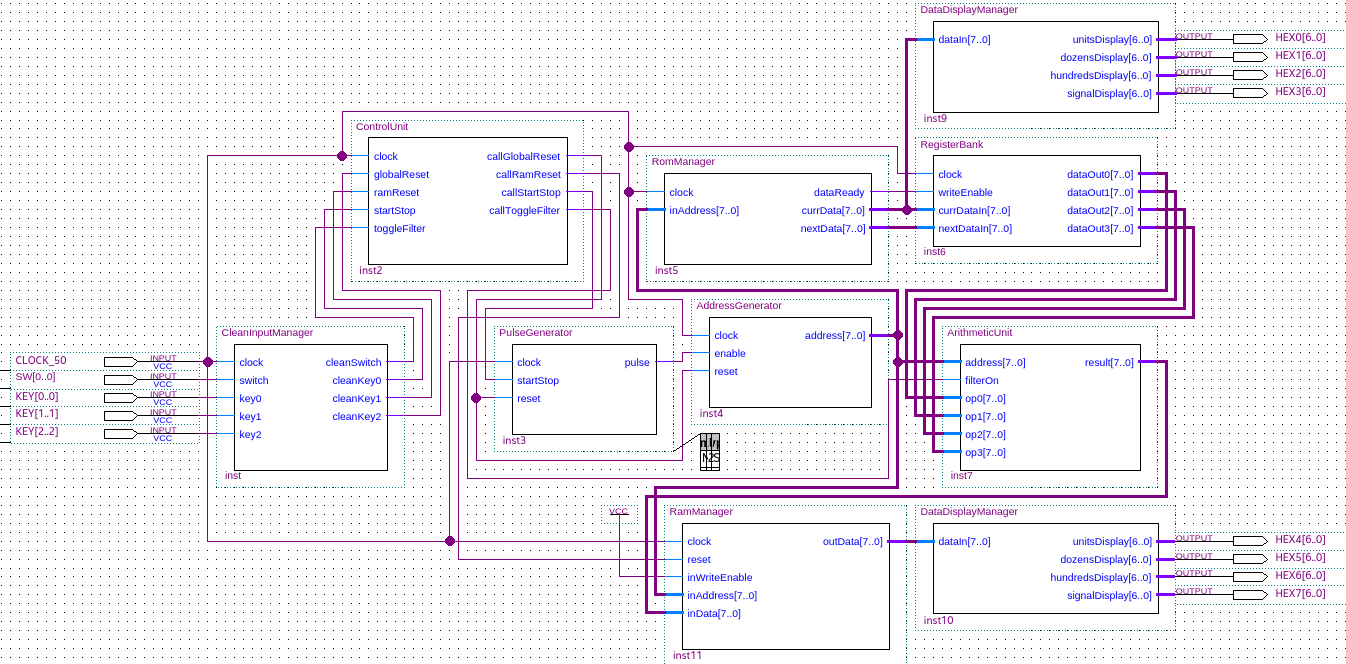
\includegraphics[width=\textwidth]{schematic.png}
    \caption{Diagrama de funcionamento do filtro de média móvel.}
\end{figure}

De uma forma simplista, o projeto é controlado por uma unidade central de controle (uma máquina de estados) que controla um gerador de endereços ligado diretamente à ROM, um registo, responsável por armazenar momentaneamente os dados obtidos da ROM e enviá-los para uma unidade aritmética  capaz de efetuar os cálculos de filtragem do sinal recebido da ROM. Em seguida, este sinal devidamente filtrado é guardado na RAM.

Tanto os valores armazenados na ROM como os na RAM passam por módulos que os preparam para serem mostrados nos displays de 7 segmentos do kit Terasic DE2-115 como números inteiros com sinal em base 10.

\subsection*{CleanInputManager}

Componente responsável pela sincronização e remoção de interferências mecânicas provenientes dos sinais das keys e dos switches. Optou-se por juntar os DebounceUnit e o sincronizador de forma a simplificar o top-level do projeto.

\subsection*{ControlUnit}

Componente responsável pelo comportamento das restantes entidades. Este trata-se de uma máquina de estados que suporta os seguintes estados:
\begin{itemize}
    \item t\_GlobalReset: efetua o reset dos componentes essenciais (PulseGenerator e AddressGenerator) e avança para o estado t\_RAMRESET.
    \item t\_RAMRESET: efetua o reset da memória RAM escrevendo todos os endereços com x"00" preservando o endereço anterior. Se for executado enquanto o sistema estiver no estado t\_STOPPED, mantém esse mesmo estado após o reset. Se for executado enquanto o sistema estiver no estado t\_RUNNING, mantém esse mesmo estado após o reset. Numa primeira execução (quando o estado anterior é t\_GlobalReset) passa ao estado t\_RUNNING.
    \item t\_RUNNING e t\_STOPPED: permite a geração ou bloqueio da geração de endereços.
\end{itemize}

\begin{figure}[H]
    \centering
    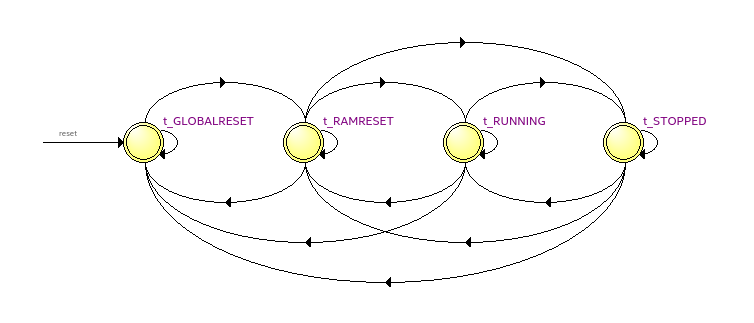
\includegraphics[width=\textwidth]{controlunit.png}
    \caption{Diagrama de estados da ControlUnit.}
\end{figure}

\subsection*{RomManager}

Entidade responsável por obter o valor do endereço atual e o valor do próximo endreço. Tem como por base uma máquina de estados de 4 estados:

\begin{itemize}
    \item t\_IDLE: mantém-se neste estado até haver uma alteração de endereço. Quando esta mudança ocorre, avança para t\_CURRADDRESS.
    \item t\_CURRADDRESS: obtém o valor gurdado na memória ROM no endereço atual, avançando para o estado t\_NEXTADDRESS.
    \item t\_NEXTADDRESS: gera o próximo endereço e obtém o valor guardado na memória ROM nesse endereço, avançando para o estado t\_DATAREADY.
    \item t\_DATAREADY: gera um pulso indicando que já obteve o valor atual e o próximo valor e regressa ao estado t\_IDLE.
\end{itemize}

\begin{figure}[H]
    \centering
    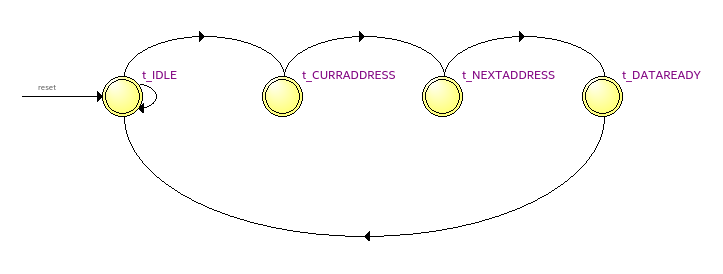
\includegraphics[width=\textwidth]{rommanager.png}
    \caption{Diagrama de estados da RomManager.}
\end{figure}

\subsection*{RamManager}

Componente responsável por efetuar o reset à memória RAM através de um gerador de endereços interno, independente do gerador de endereços principal, o que permite que o endereço seja preservado.

Optou-se por encapsular a memória RAM neste componente de forma a simplificar o top-level do projeto.

\section*{Validações}
\label{chap.validacoes}

Nesta secção estão as simulações dos compontentes mais importantes do processo de filtragem assim como a testagem do projeto.

\begin{figure}[H]
    \centering
    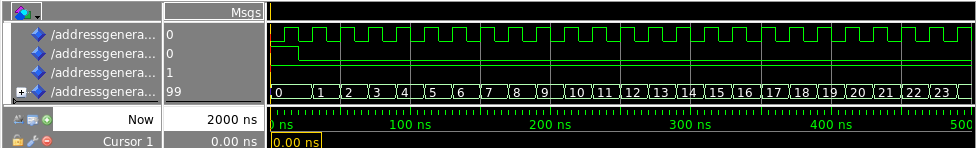
\includegraphics[width=\textwidth]{addressgeneratorval.png}
    \caption{Simulação do gerador de endereços.}
\end{figure}

\begin{figure}[H]
    \centering
    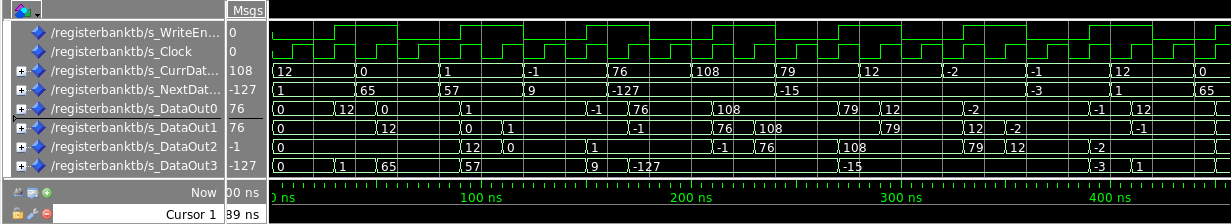
\includegraphics[width=\textwidth]{registerbankval.png}
    \caption{Simulação do RegisterBank.}
\end{figure}

\begin{figure}[H]
    \centering
    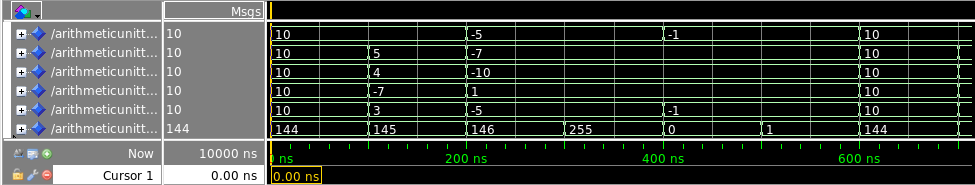
\includegraphics[width=\textwidth]{arithmeticunitval.png}
    \caption{Simulação da ArithmeticUnit.}
\end{figure}

\begin{figure}[H]
    \centering
    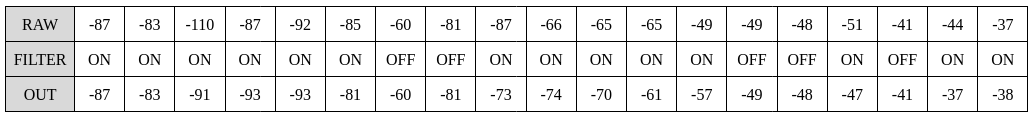
\includegraphics[width=\textwidth]{values.png}
    \caption{Testagem dos valores de saída do projeto.}
\end{figure}

\section*{Conclusão}
\label{chap.conclusao}

Tal como esperado, consegui-se realizar o projeto implementando todas as funcionalidades pedidas no enunciado. Todas as dificuldades encontradas no processo de planeamento e desenvolvimento foram superadas como fruto do esforço e dedicação dos autores. Considera-se, assim, que o projeto tenha tido, no geral, boa qualidade e, por isso, autoavaliamos o projeto em 16 valores.


\section*{Contribuições dos autores}
\label{chap.contribuicoes}

Ambos os autores participaram ativamente e com empenho na realização deste projeto. Assim, este trabalho distribui-se tem uma percentagem de participação de aproximadamente 50\% para cada um dos elementos do grupo.

\end{document}